\documentclass[12pt, a4paper]{article}
\usepackage{a4wide}
\usepackage{anysize}
\usepackage[centertags]{amsmath}
\usepackage{amsfonts,amssymb,amsthm}
\usepackage{graphicx}
\usepackage{natbib}
\usepackage{wrapfig}
\usepackage{iitbieortitle}
\usepackage[english]{babel}
%\usepackage{fullpage}
%\usepackage{rotating}

\renewcommand{\baselinestretch}{1.2} %line spacing
\marginsize{1.2in}{1.2in}{1in}{1in}   %left right top bottom
%\textwidth 6in
% Title Page

\pagestyle{plain}
\def\title{DonApp : The Donate App}
\def\what{CS 699 : Software Lab}
\def\who{{ Aakrit Anshuman 193050064\\
Deepak Singh 193050074\\
Rasesh Tongia 193050015\\
Vikas Verma 193059003\\
}}
\def\guide{Prof. Kavi Arya}
\begin{document}
\titlpage
\newpage
\tableofcontents
\newpage


\section{\textbf{Main Goal Of The Project}}
The main goal of the project was to make an Android app which provides an interface for donor and needy to reach out to each other. This app can be used for displaying items which the user wants to donate. The user can post an item which is to be donated with one or more photos and a brief description of it. Any interested user in the vicinity can mark themselves as interested for any of the listed items and that item will be removed from the list. Upon viewing a product, the user will be able to see contact details and location of the owner who can be contacted and they can meet and share the items.

\section{\textbf{Motivation}}
We can find numerous examples of donation for natural calamities and major incidents such as for floods, earthquakes, prime minister relief fund, etc. But nothing such is available on an individual level. Our vision is to provide a platform for donation of everyday use objects which could serve a better purpose in new hands.


\section{\textbf{Prior Work}}
 There is no such app available on an Individual level but there are some Donation apps available for community benefit.Some of them are:
 \begin{itemize}
     \item ShareTheMeal - An app by UN for fighting global hunger
     \item Charity Miles - An app which funds a charity on the basis of how much we run/walk/cycle
     \item Make a Stand App - An app which enables us to crowdfund for social campaign
     \item Friends2Support - App which allows location based voluntary blood donation.
    \item Donate a Photo by Johnson Johnson - An app which donates \$1 for every photo we donate.

 \end{itemize}
\newpage
\section{\textbf{Requirements for App}}
User's System Requirements are:
\subsection{Hardware}
A smartphone with the following features:
\begin{itemize}
    \item 2 GB of RAM
    \item 1 Ghz Processing Power
\end{itemize}
\subsection{Software}
\begin{itemize}
    \item Android 8.0 (Oreo) or Higher
\end{itemize}
\section{Development Environment and Tools used}
\subsection{Hardware}
A personal computer with the following configurations were used:
\begin{itemize}
    \item 8 GB of RAM
    \item 2.5 Ghz Processor
\end{itemize}
\subsection{Tools and Environment}
The softwares and tools used are:
\begin{itemize}
    \item Windows 10 Home
    \item Ubuntu 18.04
    \item Android Studio 3.5.1
    \item \LaTeX (Using Overleaf)
    \item Google Chrome
    \item Xampp / Lampp for hosting the servers
\end{itemize}
\subsection{\textbf{Programming Languages}}
\begin{itemize}
    \item Java 
    \item Php
    \item XML
    \item SQL
\end{itemize}
\section{\textbf{Features}}
\begin{itemize}
    \item User can add an item to the list along with a photo
    \item User can see details of items and mark it for taking
    \item User can search the list for an item
    \item User can refresh page
    \item There is a fixed count of how many items a user can take in a month so as to prevent abuse
\end{itemize}
\section{\textbf{User Documentation}}
\subsection{UI Details}
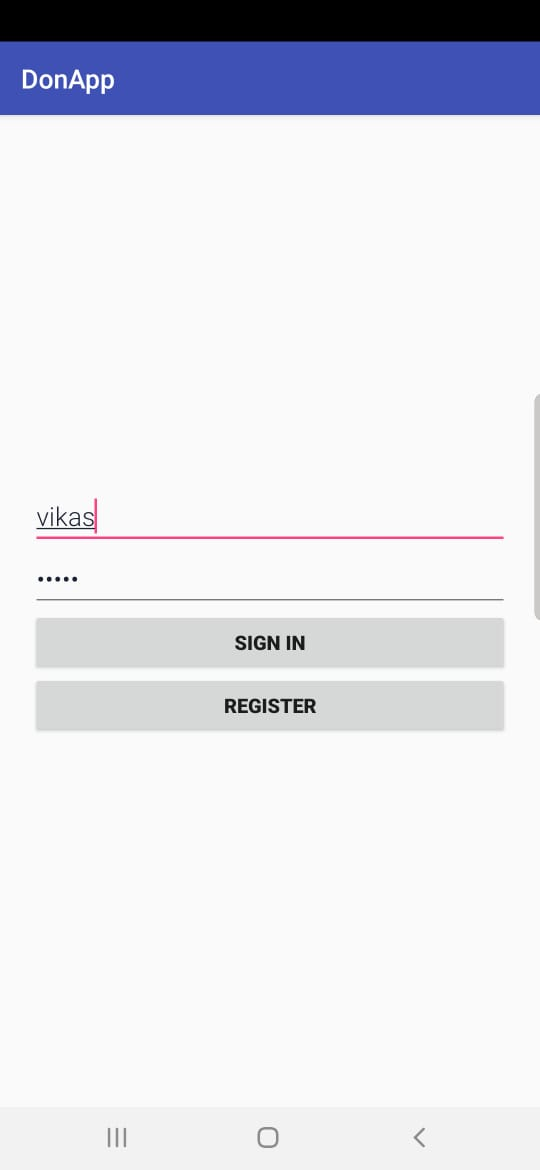
\includegraphics[width=5cm, height=8cm]{login.jpeg}
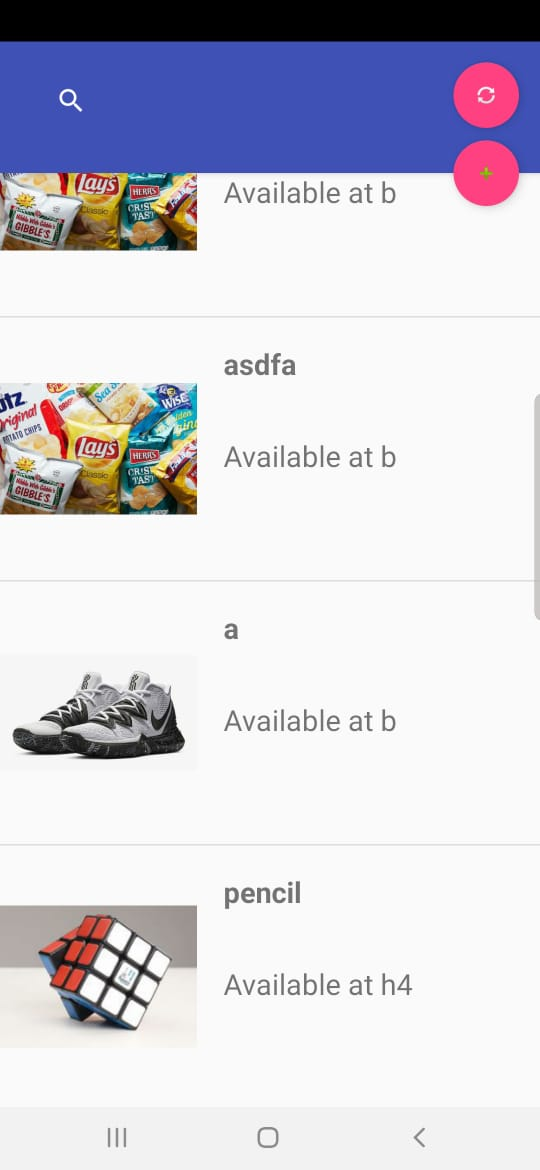
\includegraphics[width=5cm, height=8cm]{list.jpeg}
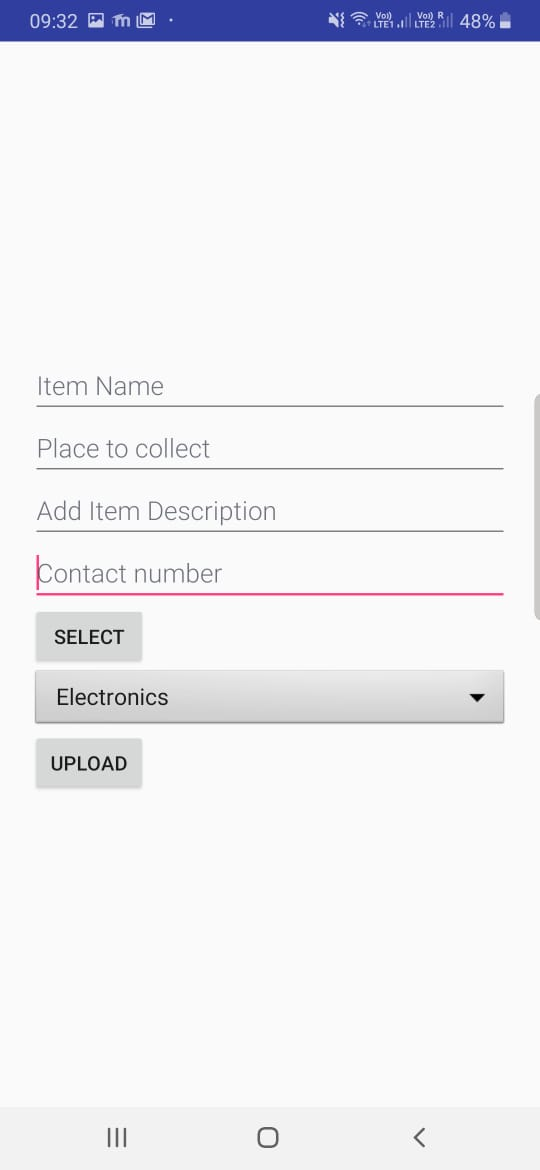
\includegraphics[width=5cm, height=8cm]{additem.jpeg}
\newline
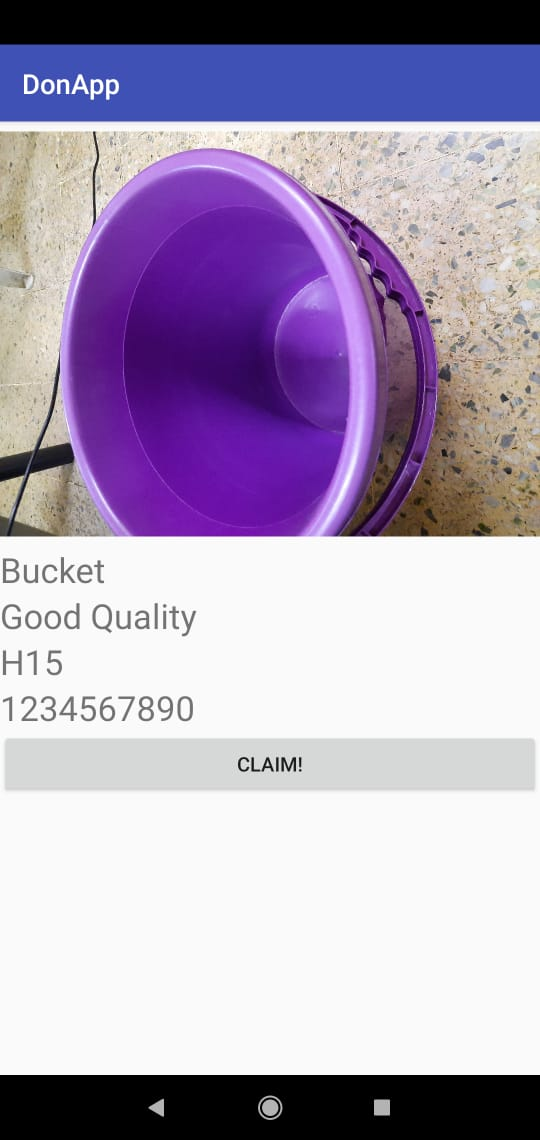
\includegraphics[width=5cm, height=8cm]{bucket.jpeg}
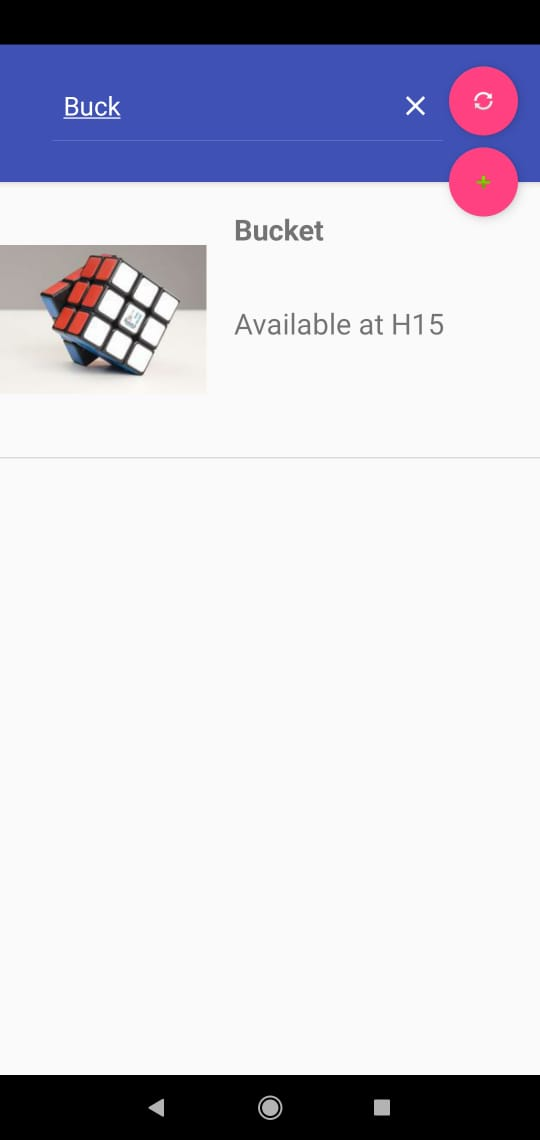
\includegraphics[width=5cm, height=8cm]{search.jpeg}
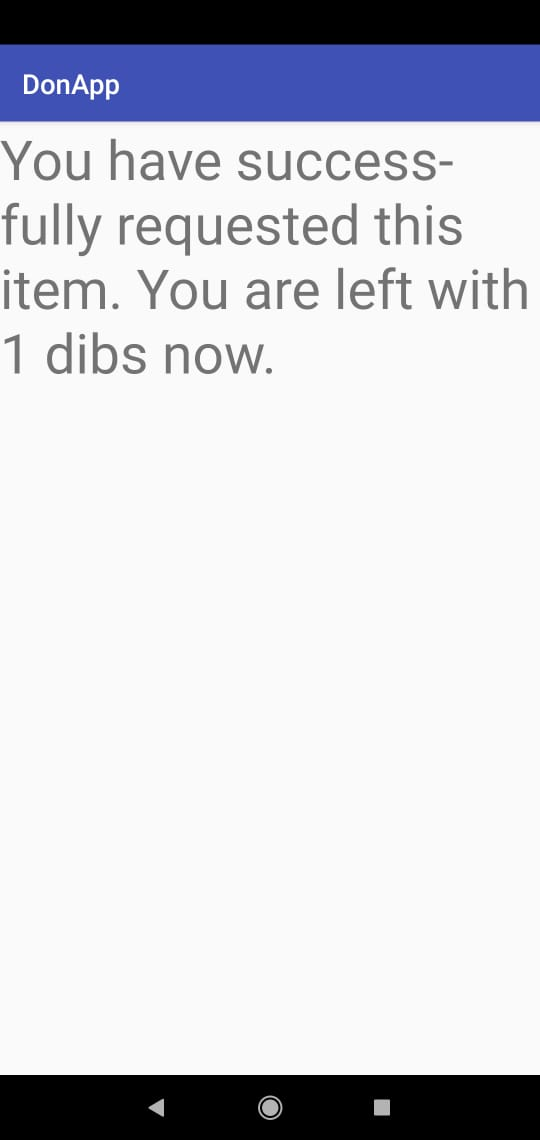
\includegraphics[width=5cm, height=8cm]{dibs.jpeg}

\subsection{Server Setup}
We are using Xampp (For Windows) / Lampp (For Linux) to maintain our server. 
The steps for setting up the server are as follows:
'\begin{enumerate}
    \item Download and install Xampp from the following link https://www.apachefriends.org/ download.html
    \item For Windows: Open Xampp Control Panel from the directory where Xampp was installed.
    \begin{enumerate}
        \item In the Xampp control panel, start the modules for 'Apache' and 'MySQL'
        \item After both the modules have started, click on 'Admin' button for 'Apache' module.
        \item A webpage will open up in the browser. Click on the tab 'phpMyAdmin' (usually on the top right).
    \end{enumerate}
    \item For Linux: Go to the directory /opt/lampp and run the command: sudo ./xampp start
    \begin{itemize}
        \item In a browser open localhost/phpmyadmin
    \end{itemize}
    \item On the left click on option 'new' to create a new database. Name the database as 'firstDB'.
    \item Click on the icon for newly created Database 'firstDB' and go to the 'SQL' tab.
    \item Type the following commands and click on Go:
    \begin{itemize}
        \item CREATE TABLE `itemlist` (`item\_id` int(11) NOT NULL, `item\_name` varchar(30) NOT NULL, `place` text NOT NULL DEFAULT 'IITB', `image\_path` text NOT NULL, `description` text NOT NULL DEFAULT 'No further info', `contact` varchar(20) NOT NULL DEFAULT '0', `category` enum('Education','Sports','Food','Clothing','Footwear', 'Stationary','Others') NOT NULL DEFAULT 'Others', `donorid` text NOT NULL DEFAULT '0,  `doneeid` text NOT NULL DEFAULT '0', `status` enum('added', 'requested','approved','') NOT NULL DEFAULT 'added')
        \item CREATE TABLE `users` ( `id` int(20) NOT NULL, `username` varchar(70) NOT NULL, `password` varchar(40) NOT NULL, `email` varchar(50) NOT NULL, `dibscount` int(11) NOT NULL DEFAULT 0, `created\_at` datetime NOT NULL, `updated\_at` datetime DEFAULT NULL)
    \end{itemize}
    \item Run the following command in terminal / command prompt for enabling http server to respond to image requests
    \begin{itemize}
        \item ruby -run -ehttpd . -p8000
        [2019-11-27 08:44:40] INFO  WEBrick 1.4.2 
        [2019-11-27 08:44:40] INFO  ruby 2.5.1 (2018-03-29) [x86\_64-linux-gnu]
        [2019-11-27 08:44:40] INFO  WEBrick::HTTPServer\#start: pid=5175 port=8000
    \end{itemize}
    \item Find out the IP address of the system where the Xampp is being run. Use the commands 'ipconfig' in Windows Command Prompt Shell or 'ifconfig' in Linux to obtain the IP addresses.
    \item Copy the IP address to the java file in the path: \textasciitilde \textbackslash DonApp-master\textbackslash DonApp\textbackslash src\textbackslash main \textbackslash java\textbackslash com\textbackslash journaldev\textbackslash DonApp\textbackslash ipaddress.java in the static String variable 'ipadd'.
    \item We use Android Studio which can be downloaded from https://developer.android.com/studio
    \item After installing Android Studio, download SDK for Android 8.0 (api 24)
    \item The entire folder 'Donapp-master' should be used as a project for Android Studio.
    \item Build and Run the Project. The apk file can be made from here and installed in any smartphone for usage.
\end{enumerate}
\section{\textbf{Feasibilty}}
The feasibility details are as follows:
\subsection{Economic Feasibility}
The app was economically feasible to make as no costs were involved in making it.
\subsection{Technical Feasibility}
With the tools that are available, GUI with back-end integration was feasible to be made.
\subsection{Legal Feasibilty}
The data collected from the user is not misused or shared with a third party and so it is legally feasible.

\section{Outcome}
The outcomes of this project is that it can be used in real life within IIT Bombay as well as outside (with a few modifications) so that something which is no longer useful to a person can be donated to someone who finds it useful.

\begin{thebibliography}{9}
\bibitem{apps} www.mdgmonitor.org/top-5-donation-appssharethemeal-charity-miles/
\bibitem{blood donation} ieeexplore.ieee.org/document/7988025
\bibitem{smartphone apps} www.thebalancesmb.com/give-to-charity-every-day-with-these-6-smartphone-apps-3861763
\end{thebibliography}
\end{document}